\section{Software Design of REACH}
In addition to the hardware implementation by selecting appropriate force sensors and locating them in the appropriate places around the mobile device, we also build the classifier for the hand grip. In this section, we discuss how we collect force sensor values from mobile device for training and how we implement the classifier for grip pattern detection. We then used the model to predict the pattern in realtime manner.
\par
For training the model,  we used the Weka (Witten \& Frank 2005) machine learning library for Java. We used Bayesian network, Support vector machine and Classification tree algorithms for training the model on the collected data. We performed off-line training on a laptop and extracted the parameters of the best model to implement the realtime version of REACH.

\subsection{Tap Detection as Proxy}
While waiting for the hardware to be completed, we decided to perform some experiments to provide insight into how to  classify the grip patterns. Tap detection was chosen as a proxy for grip pattern detection. We used the accelerometer data available from an Android phone to try and classify instances when a user performs a single tap on the back of the device.
\par
The accelerometer data from 3 axis (x, y, z) is analogous to the force data available from the 16 sensors for grip detection. Similarly, both accelerometer and force data will change when an action is performed by the user. The only difference is that the accelerometer data changes depending on the orientation of the phone, while the force data is unaffected. To mitigate this, all data collected and analyzed for tap detection focused on keeping the phone in portrait orientation, the y-axis facing away from the floor and the z-axis facing towards the user.

\subsubsection{Determine Window Size}
The Android sensor collects accelerometer data on a periodic basis. This sampling interval is neither guaranteed nor specified by the Android SDK, but using the default mode, it was found to be 20ms on \textit{average}. After analyzing the data, it was noticed that the characteristic pattern of a single tap lasted for a duration of 400ms on average. This duration is defined as the \textit{window duration}.
\par
Dividing the window duration by the sampling interval gives us a \textit{window size} of 20. The accelerometer data is partitioned into windows with the specifications above, and implemented as a \textit{sliding window}. This means that the starting time for each subsequent window differs by the sampling interval. Contrast this against a \textit{jumping window}, where the start time for subsequent windows would be the window duration. Using the \textit{sliding window} protocol ensures that a possible tap is not missed during the evaluation process.
\par
Picking the right window size is crucial since it has a direct impact on the accuracy of the classification model. If the \textit{window size} is too small, then the complete characteristic pattern of a tap will not be captured, leading to incorrect classifications. However, using a window size that is too large will capture extraneous noisy data that will also reduce the classification accuracy. This topic will again be explored for grip pattern detection.

\subsubsection{Determine Features}
Upon observing the data, it was noticed that acceleration values of the x, y and z axis all changed when the tap action was performed. The \textit{inter}-window change was captured by calculating the \textit{mean} for a window, and this was used as one of the features for training the model. There was a visible change in the acceleration values within the window duration, and this \textit{intra}-window change was represented by calculating the \textit{variance} of a window.

\subsubsection{Classify a Tap}
Even though a windowing principle was used, windows clustered near a tap duration all show a similar characteristic pattern, albeit time-shifted. Therefore while performing the manual classification of the training data, we decided to label, on average, 20 windows as a single tap. This means that when a tap is being evaluated with real-time data, we would expect 20 back-to-back windows all to be predicted as a tap. Once such a scenario is detected, we would report a successful tap as being detected.

\subsubsection{Tap Model Performance}
We collected acceleration values of the x, y, and z dimension of three different activities on the mobile: \emph{None}, \emph{Motion}, and \emph{Tap}. The mean and variance of each window for each dimension is then calculated and are used as instance features for training a model. The Motion activity is added to represent the boundary between Tap and None activities.  The corresponding activity of each window is labeled manually (\emph{i.e.}, None, Motion, and Tap) and used as class feature for training a model. 
\par
We used Bayesian network, Naive bayes and Support vector machine algorithms with Weka's default configuration for training. We also used different number of instances with different ratios between class features. In all cases, Bayesian network was the winner among other algorithms. Table \ref{tbl-Confusion Matrix} shows the confusion matrix of using Bayesian network algorithm with 10-fold cross validation of 2250 instances (among them are 1000 None, 1000 Motion, and 250 None instances). The matrix shows that 76 of Tap activities are classified as Motion which is reasonable due to the similarity between these two activities. While 142 of Motion activities are classified as None, we believe that these are the instances which exist in the boundaries between Motion and None activities.

\begin{table}[!t]
\begin{center}
\caption{Confusion Matrix using Bayesian network with 10-fold cross validation}
\label{tbl-Confusion Matrix}
\begin{tabular}{|l||l|l|l|}\hline
        & None   & Motion   & Tap   \\ \hline \hline
None    & 970    &	29      & 1	    \\
Motion  & 142    &	825     & 33    \\
Tap     & 1      &	76      & 173	\\ \hline
\end{tabular}
\end{center}
\end{table}

\subsection{Grip Classifier}
We used the insights gained from tap detection to guide our grip classification process, namely a sliding window evaluation protocol and similar features to describe a grip pattern. We begin by attempting to classify three grip patterns in our prototype: None, Squeeze, and Reach. In None, the subject holds the device without performing any activity. In Squeeze, the subject is applying a squeeze-force on the device and in Reach, the subject is moving his thumb finger to reach the top of the device while holding the device.  
\par
The 12 force sensors around the device continuously reported data every 1 ms on average. Based on our experience with tap detection, we felt that these values could be safely aggregated into a 20ms sampling interval for the purpose of grip detection. Figure \ref{fig:window_60} shows the change in a sensors value for a \textit{window size} of 60. We can clearly see that choosing a value of 20 would result in the loss of essential information, while a value of 60 would admit noisy data. It was determined that a \textit{window size} of 50 represents the average case.

\begin{figure}[h]
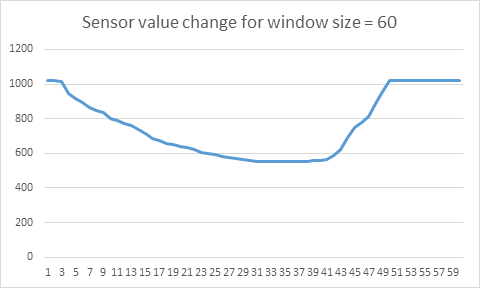
\includegraphics[width=.45\textwidth]{window_60.png}
\caption{Sensor value changes for window size 60}
\label{fig:window_60}
\end{figure}

\par
Similar to tap detection, we calculated the mean and variance for each \textit{sliding window}. It was observed that different people perform the same gesture in slightly different ways. To increase the robustness of the trained model, we decided to use the mean values of all the sensors located on one side of the device. The variance for each sensor was calculated with respect to these averaged means. For each window the following features were calculated -\textit{mean left}, \textit{mean right} and \textit{variance} for each sensor.

\subsubsection{Variability of Grip Patterns}
We wanted to establish a good baseline performance for grip pattern detection, which led us to collect all training and evaluation data from 1 subject. The individual was asked to perform Hold, Squeeze and Reach every 15 seconds for a duration of 1 minute. Each dataset collected involved repeating this process  3 times. We noticed that even for the same individual, subsequent datasets resulted in a variability of the grip patterns. The model that was trained for the first dataset performed poorly for the second dataset. However, when the second dataset was used to train the model, cross-validation performance was very similar to the original dataset. We will explore the performance further in the Evaluation section.  

